\chapter{\babDua}
\label{bab:2}
Pada bab ini dijlaskan secara rinci mengenai detil pekerjaan yang dilakukan selama program kerja praktik berlangsung. Latar belakang pekerjaan hingga hasil pekerjaan dijelaskan pada bab ini.

\section{Latar Belakang Pekerjaan}

Pelaksana kerja praktik terlibat dalam penelitian terkait manajemen klaster Kafka di Computer Systems Laboratory (CSL) Fakultas Ilmu Komputer Universitas Indonesia. Penelitian ini berfokus pada optimalisasi partisi topik untuk meningkatkan performa \textit{real-time distributed systems} berbasis Kafka. Proyek ini merupakan bagian dari penelitian bertajuk \textit{Efficient Topic Partitioning of Apache Kafka for High-Reliability Real-Time Data Streaming Applications}. Tugas pelaksana kerja praktik adalah menjalankan eksperimen yang bertujuan untuk menguji algoritma BroMax dan BroMin, yang digunakan untuk menentukan jumlah partisi optimal.

\section{Deskripsi Pekerjaan}

Pelaksana kerja praktik bertanggung jawab atas konfigurasi dan pengelolaan eksperimen \textit{end-to-end}. Proses dimulai dengan penyiapan VM di Google Cloud Platform (GCP) dan infrastruktur Universitas Indonesia (DGX dan BMKGCS), yang digunakan untuk menjalankan simulasi klaster Kafka. Tugas utama meliputi instalasi dependencies, pengaturan Kafka broker, serta analisis hasil eksperimen untuk mengukur performa sistem, khususnya \textit{throughput} dan latensi, saat algoritma BroMax dan BroMin diterapkan.

Pekerjaan dilakukan secara \textit{hybrid} dari pukul 08.00 a.m. WIB hingga pukul 12.00 p.m. WIB, dengan kehadiran di lab hanya pada hari Jumat, sedangkan hari-hari lainnya bekerja secara \textit{remote}. Hasil eksperimen dianalisis dan dilaporkan kepada dosen peneliti untuk evaluasi lebih lanjut.

\section{Tinjauan Pustaka}

Penelitian yang dilakukan selama kerja praktik ini melibatkan sejumlah konsep penting dalam pengelolaan \textit{real-time distributed systems} dengan menggunakan Apache Kafka dan teknologi pendukung lainnya. Konsep-konsep ini menjadi fondasi utama dalam penelitian dan pengembangan yang dilakukan.

\subsection{Apache Kafka}

Apache Kafka adalah platform \textit{open-source} yang dirancang untuk menangani \textit{data streaming} secara \textit{real-time} dengan \textit{throughput} tinggi dan latensi rendah. Data dibagi menjadi topik-topik yang dipartisi, sehingga memungkinkan pemrosesan paralel yang lebih efisien di seluruh klaster \citep{elsevier:kafka}. Partisi pada topik Kafka sangat penting karena memungkinkan distribusi beban kerja yang merata antar broker, sehingga meningkatkan kemampuan sistem untuk menangani data dalam jumlah besar tanpa menimbulkan \textit{bottleneck} \citep{elsevier:kafka}. Selain itu, dengan optimalisasi jumlah partisi yang tepat, \textit{throughput} sistem dapat dimaksimalkan, sehingga menjaga kinerja tinggi meskipun volume data yang diproses sangat besar \citep{elsevier:kafka}.

\subsection{Docker Containerization}

Docker Containerization adalah teknologi yang memungkinkan aplikasi dijalankan dalam \textit{container} yang terisolasi, sehingga dapat memisahkan lingkungan eksekusi aplikasi dari sistem \textit{host}. Docker memungkinkan konsistensi lingkungan, meminimalkan konflik konfigurasi, serta meningkatkan portabilitas sistem \citep{its:docker}. Dengan Docker, seluruh proses \textit{deployment} Kafka menjadi lebih efisien karena setiap \textit{node} dalam klaster dapat dijalankan dengan konfigurasi yang seragam, sehingga mengurangi kesalahan operasional \citep{its:docker}.

\subsection{Apache Zookeeper}

Apache Zookeeper adalah layanan koordinasi terpusat yang digunakan untuk mengelola \textit{metadata} dan menjaga konsistensi di dalam klaster Kafka. Zookeeper bertugas mengatur eleksi pemimpin partisi, menyinkronkan data antar broker, serta memastikan bahwa setiap perubahan dalam klaster Kafka ditangani dengan cepat dan efisien \citep{comp:zookeeper}. Dalam konteks Kafka, Zookeeper memainkan peran penting dalam memastikan bahwa sistem tetap \textit{fault-tolerant}. Jika terjadi kegagalan pada salah satu broker, Zookeeper secara otomatis memilih broker lain untuk menjadi pemimpin, sehingga menjaga kestabilan sistem \citep{comp:zookeeper}. Zookeeper juga menyimpan informasi konfigurasi mengenai topik dan partisi Kafka, dan memastikan bahwa produser dan konsumen dapat berinteraksi dengan sistem secara konsisten \citep{comp:zookeeper}.

\subsection{Distributed System}

Distributed System adalah sistem yang terdiri dari beberapa \textit{node} yang terhubung dan bekerja bersama untuk mencapai tujuan tertentu. Dalam konteks Kafka, sistem terdistribusi ini memastikan bahwa data dapat diolah secara paralel dan skalabel di berbagai broker yang tersebar dalam klaster. Keunggulan dari sistem terdistribusi seperti Kafka adalah kemampuannya untuk tetap berfungsi meskipun terjadi kegagalan pada satu atau beberapa \textit{node} dalam klaster \citep{ieee:distributed}. Dalam sistem terdistribusi Kafka, partisi topik didistribusikan ke berbagai broker, sehingga meningkatkan ketersediaan data dan mempercepat proses pengiriman data dari produser ke konsumen \citep{ieee:distributed}. Sistem ini juga memungkinkan replikasi data secara otomatis, di mana salinan data disimpan di beberapa broker untuk meningkatkan keandalan dan redundansi sistem \citep{ieee:distributed}.

\section{Metodologi Pekerjaan}

Selama pelaksanaan kerja praktik, penelitian dilakukan dengan metodologi yang berfokus pada eksperimen \textit{end-to-end} yang bertujuan untuk memantau dan menganalisis perilaku \textit{real-time distributed systems} menggunakan Apache Kafka. Tahapan pekerjaan yang dilaksanakan secara bertahap sesuai dengan proses yang dirancang, mulai dari pengaturan infrastruktur hingga analisis hasil eksperimen. Berikut adalah tahapan metodologi pekerjaan yang dilakukan selama kerja praktik:

\begin{enumerate}

	\item \textbf{Pengaturan VM (VM Setup)} Langkah awal dalam kerja praktik ini adalah menyiapkan VM (Virtual Machine) di Google Cloud Platform (GCP). VM tersebut dikonfigurasi menggunakan SSH dengan akses root. Setelah VM disiapkan, seluruh dependensi yang diperlukan untuk menjalankan eksperimen Kafka diinstal. Konfigurasi ini memastikan bahwa VM siap untuk menjalankan berbagai eksperimen Kafka, di mana satu VM bertindak sebagai Kafka client, dan VM lainnya berperan sebagai Kafka cluster. Seluruh pengaturan ini bertujuan untuk mendukung kelancaran eksperimen yang dilakukan.

	\item \textbf{Eksekusi Eksperimen (Experiment Execution)} Setelah pengaturan infrastruktur selesai, eksperimen dilakukan dengan fokus pada simulasi \textit{end-to-end} yang bertujuan untuk memantau algoritma BroMax dan BroMin dalam menentukan jumlah partisi dan broker pada sistem Apache Kafka. Eksperimen ini melibatkan pengaturan dua VM dengan fungsi yang berbeda: satu VM bertindak sebagai Kafka client yang mengirimkan dan menerima data, sedangkan VM lainnya bertindak sebagai Kafka cluster berisi broker yang mengelola partisi. Eksperimen ini penting untuk memahami perilaku \textit{throughput} dan latensi sistem secara keseluruhan dalam kondisi yang mendekati \textit{real-time streaming}. Hasil dari eksperimen ini memberikan wawasan tentang cara kerja algoritma BroMax dan BroMin dalam optimasi partisi.

	\item \textbf{Pemantauan Sumber Daya (Resource Monitoring)} Selama eksperimen berlangsung, pemantauan sumber daya dilakukan secara berkala untuk memantau penggunaan CPU, RAM, dan \textit{disk space} pada VM. Hal ini penting untuk memastikan bahwa eksperimen berjalan dengan efisien tanpa ada \textit{bottleneck} dalam pemanfaatan sumber daya. Data yang dihasilkan dari pemantauan sumber daya ini juga menjadi acuan dalam mengevaluasi performa algoritma BroMax dan BroMin.

	\item \textbf{Eksperimen Infrastruktur UI (UI Infrastructure Experiments)} Setelah eksperimen di GCP berhasil dilaksanakan, eksperimen serupa diulang pada infrastruktur UI menggunakan mesin DGX dan BMKGCS. Eksperimen ini dilakukan untuk memastikan bahwa hasil eksperimen dapat direplikasi di lingkungan yang berbeda dengan kapasitas sumber daya yang lebih besar. Selain itu, eksperimen ini juga mengeksplorasi penggunaan teknologi Docker-in-Docker (DinD) untuk menjalankan eksperimen tanpa akses root pada mesin infrastruktur UI. Pendekatan ini memberikan fleksibilitas lebih dalam menjalankan eksperimen di lingkungan yang lebih terbatas.

	\item \textbf{Implementasi Docker (Docker Implementation)} Dalam eksperimen ini, Docker digunakan untuk membangun dan mengelola \textit{container} yang berisi aplikasi Apache Kafka. Pelaksana kerja praktik mempelajari cara kerja Docker, mulai dari membangun image hingga pengaturan komunikasi antar \textit{container}. Implementasi Docker ini bertujuan untuk memudahkan manajemen infrastruktur eksperimen dengan memisahkan setiap komponen sistem ke dalam container yang terisolasi. Selain itu, penggunaan Docker juga meminimalkan masalah yang mungkin terjadi dalam konfigurasi VM dan meningkatkan portabilitas sistem.

	\item \textbf{Analisis Data dan Pelaporan (Data Analysis and Reporting)} Setelah seluruh eksperimen selesai dijalankan, data hasil eksperimen dianalisis untuk membuat plot yang menggambarkan performa \textit{throughput} dan latensi sistem. Plot ini kemudian digunakan untuk mendeskripsikan perilaku algoritma BroMax dan BroMin dalam kondisi eksperimen yang telah dilakukan. Hasil analisis ini kemudian disajikan dalam laporan kepada dosen peneliti, serta didiskusikan dengan para peneliti lainnya untuk mendapatkan umpan balik dan evaluasi lebih lanjut mengenai hasil eksperimen.

\end{enumerate}

\section{Teknologi}

Selama pengerjaan proyek pada kerja praktik, beberapa teknologi utama digunakan untuk mendukung penelitian. Berikut adalah teknologi-teknologi tersebut:

\begin{itemize}

	\item \textbf{Apache Kafka}, Sebuah platform yang digunakan untuk memproses data secara paralel dan \textit{real-time} melalui topik yang dipartisi. Kafka memungkinkan penanganan volume data yang sangat besar dengan \textit{throughput} tinggi dan latensi rendah, serta mendukung replikasi data untuk menjaga keandalan sistem.

	\item \textbf{Docker}, Merupakan platform \textit{containerization} yang memungkinkan pengembang menjalankan aplikasi dalam lingkungan terisolasi yang disebut container. Docker digunakan untuk menyederhanakan \textit{deployment} sistem Apache Kafka dan komponen lainnya selama eksperimen. Docker memastikan lingkungan yang seragam dan memudahkan migrasi antar infrastruktur.

	\item \textbf{Linux}, Sistem operasi \textit{open-source} yang digunakan dalam menjalankan berbagai komponen pada infrastruktur server. Linux menawarkan stabilitas dan kontrol penuh terhadap manajemen sumber daya, yang sangat penting untuk menjalankan aplikasi terdistribusi seperti Kafka dan Docker.

	\item \textbf{Bash}, Bash adalah bahasa skrip yang digunakan untuk mengotomatisasi berbagai tugas di lingkungan Linux. Dalam proyek ini, Bash digunakan untuk menjalankan skrip yang mengelola proses \textit{deployment}, \textit{system monitoring}, dan pemeliharaan sumber daya.

	\item \textbf{Python}, Sebuah bahasa pemrograman yang digunakan untuk menulis skrip otomasi dan pengolahan data. Python sangat fleksibel dan mendukung banyak \textit{library} untuk analisis data, pemantauan sistem, dan integrasi dengan platform lain seperti Kafka.

	\item \textbf{Google Cloud Platform (GCP)}, GCP adalah platform komputasi awan yang menyediakan infrastruktur untuk menjalankan VM yang mendukung eksperimen Kafka. GCP digunakan untuk skala dan fleksibilitas, memungkinkan pengembang menguji aplikasi di lingkungan cloud yang efisien.

	\item \textbf{WhatsApp}, Sebagai aplikasi perpesanan, WhatsApp digunakan dalam konteks komunikasi informal antara tim dan dosen peneliti selama proyek.

\end{itemize}

\section{Hasil Pekerjaan}

Selama periode kerja praktik, pelaksana terlibat dalam tugas-tugas yang menuntut analisis mendalam terkait {real-time data streaming} menggunakan Apache Kafka. Pada bagian ini dijelaskan tugas apa saja yang sudah diselesaikan pada periode kerja praktik berlangsung.

\subsection{Framework untuk Melakukan Eksperimen}

Selama kerja praktik, pelaksana kerja praktik menghadapi kendala signifikan terkait \textit{experiment setup} dengan klaster Kafka, terutama saat memindahkan eksperimen dari satu \textit{host} ke \textit{host} lain. Setiap kali berpindah lingkungan, diperlukan pengaturan ulang VM dan pengunduhan dependensi, yang memakan waktu dan rentan terhadap kesalahan manusia. Hal ini sering mengganggu alur eksperimen dan menghambat analisis lebih lanjut.

Untuk mengatasi masalah ini, pelaksana kerja praktik mengusulkan ide kepada dosen peneliti untuk mengembangkan \textit{framework}. \textit{Framework} ini dirancang agar dapat mengotomatisasi seluruh proses \textit{setup}, sehingga pengguna hanya perlu menjalankan sedikit skrip tanpa perlu mengulang pengaturan secara manual. Dengan adanya \textit{framework} ini, pelaksana kerja praktik dapat langsung fokus pada analisis eksperimen tanpa harus khawatir tentang masalah teknis terkait lingkungan yang berulang kali harus disesuaikan. \textit{Framework} ini dapat diakses oleh siapa saja melalui \href{https://github.com/bryan-ilman-on-github/kafka-part-exp}{https://github.com/bryan-ilman-on-github/kafka-part-exp}.

\subsection{Analisis Eksperimen End-To-End}

\begin{figure}
	\centering
	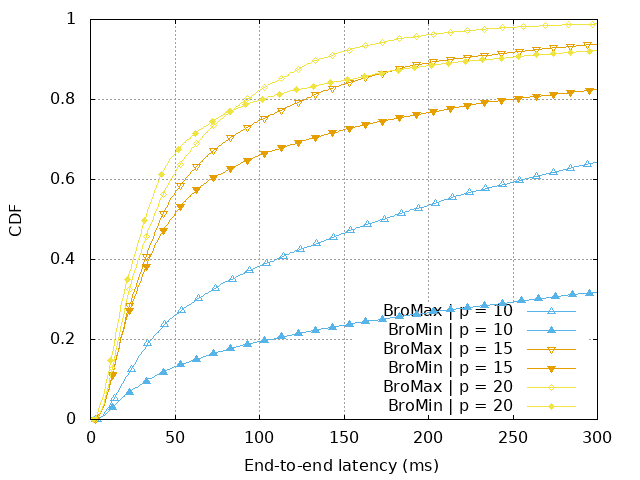
\includegraphics[width=1\textwidth]
	{assets/pics/003-latency-cdf.png}
	\caption{Analisis Eksperimen \textit{End-To-End}}
	\label{fig:latency-cdf}
\end{figure}

Salah satu temuan utama dari eksperimen ini adalah bahwa metode penentuan jumlah partisi sangat memengaruhi \textit{throughput} dan latensi: Terlihat pada \pic~\ref{fig:latency-cdf} bahwa algoritma BroMax, yang aktif memaksimalkan penggunaan semua sumber daya yang tersedia untuk mendistribusikan beban kerja, berhasil mempertahankan latensi yang rendah sehingga menghasilkan \textit{throughput} yang relatif lebih tinggi. Sebaliknya, algoritma BroMin, yang lebih konservatif dalam penggunaan sumber daya, cenderung memiliki latensi yang sedikit lebih tinggi, sehingga \textit{throughput}-nya relatif lebih rendah.

Selain itu, terlihat pula pada \pic~\ref{fig:latency-cdf} bahwa jumlah produsen yang lebih banyak justru mengurangi latensi secara keseluruhan, berlawanan dengan intuisi awal yang menganggap bahwa lebih banyak produsen akan meningkatkan beban klaster dan menyebabkan latensi lebih tinggi. Setelah diskusi dengan tim, didapat penjelasan untuk temuan ini bahwa tingginya \textit{overhead} pada klaster dengan sedikit produsen tidak ideal untuk beban kerja yang sebenarnya. Sebaliknya, pada klaster dengan lebih banyak produsen, \textit{overhead} menjadi tidak signifikan dibandingkan dengan beban kerja yang ada, sehingga performanya lebih stabil. Hasil eksperimen ini memberikan wawasan yang lebih mendalam tentang pengoptimalan konfigurasi klaster Kafka.

\section{Aspek Non Teknis}

Dalam pelaksanaan kerja praktik, terdapat berbagai pembelajaran non-teknis yang turut berperan penting dalam mendukung keberhasilan tugas. Aspek-aspek seperti komunikasi dan kerja sama tim menjadi bagian integral dari keseluruhan pengalaman kerja praktik.

\subsection{Komunikasi}

Selama kerja praktik, komunikasi memainkan peranan yang sangat penting dalam memastikan kelancaran proyek dan kesesuaian hasil dengan tujuan yang ditetapkan. Salah satu contoh penting dalam hal ini adalah komunikasi yang dilakukan melalui email dengan Profesor Claudio Cicconetti dari Università di Pisa, penulis penelitian yang eksperimennya sedang pelaksana kerja praktik coba untuk replikasi. Pelaksana kerja praktik menghubungi Profesor Cicconetti untuk meminta klarifikasi mengenai beberapa aspek teknis dari penelitiannya, dan beliau dengan ramah memberikan tanggapan serta penjelasan yang sangat membantu. Hal ini menekankan pentingnya komunikasi yang efektif dalam lingkungan akademik dan profesional, terutama saat bekerja dengan pihak eksternal yang memiliki keahlian khusus dalam bidang tertentu.

\subsection{Kerja Sama Tim}

Kerja sama tim merupakan aspek lain yang sangat penting dalam pelaksanaan proyek selama kerja praktik. Dalam mengerjakan proyek, tidak ada tugas yang dilakukan sepenuhnya secara mandiri. Setiap anggota tim memiliki peran spesifik yang saling berhubungan, dan keberhasilan satu bagian proyek sering kali tergantung pada penyelesaian bagian lain yang dikerjakan oleh anggota tim lain.

\section{Analisis Pelaksanaan Kerja Praktik}

Pada bagian ini dijelaskan analisis menyeluruh mengenai pelaksanaan kerja praktik. Penjelasan dimulai dengan mengkaji kesesuaian pelaksanaan kerja praktik terhadap kerangka acuan kerja praktik yang telah disusun. Selain itu, kendala-kendala yang muncul selama kerja praktik berlangsung juga akan diuraikan, beserta solusi yang diterapkan untuk mengatasi hambatan tersebut.

\subsection{Ulasan kesesuaian dan perbedaan dengan KAKP}

Secara keseluruhan, pelaksanaan kerja praktik telah berjalan sesuai dengan yang tercantum dalam Kerangka Acuan Kerja Praktik (KAKP). Semua target yang telah ditetapkan terlaksana dengan baik, dan tidak ada permintaan yang melebihi apa yang telah diuraikan dalam KAKP.

\subsection{Ulasan tentang kendala dan cara menanganinya}

Selama kerja praktik, beberapa kendala teknis muncul, berkaitan langsung dengan pekerjaan yang dilakukan. Setiap kendala yang ada diatasi dengan solusi yang sesuai untuk memastikan eksperimen tetap berjalan lancar.

\subsubsection{Tidak Memiliki Akses Root pada Infrastruktur UI}

Salah satu kendala utama yang muncul selama kerja praktik adalah keterbatasan akses root pada infrastruktur Universitas Indonesia (UI). Akses root sangat penting dalam eksperimen, terutama untuk mengunduh \textit{library} atau melakukan konfigurasi yang lebih mendalam pada sistem. Tanpa akses ini, beberapa langkah teknis yang memerlukan izin tingkat sistem tidak dapat dilakukan secara langsung, sehingga menghambat kelancaran eksperimen. Kondisi ini menuntut solusi yang inovatif untuk mengatasi batasan tersebut.

Untuk mengatasi kendala ini, diterapkan solusi Docker-in-Docker (DinD), yang memungkinkan pengunduhan dan instalasi \textit{library} secara independen di dalam container Docker. Pendekatan ini sangat efektif karena dengan menggunakan DinD, dapat dibuat lingkungan isolasi tambahan yang tidak memerlukan akses root langsung pada mesin \textit{host}.

\subsubsection{Dokumentasi dari Peneliti Asli Kurang Lengkap atau Usang}

Kendala lain yang dihadapi adalah dokumentasi penelitian asli yang tidak lengkap atau sudah usang. Dokumentasi dari penelitian yang direplikasi sering kali tidak menyertakan penjelasan yang detail mengenai setiap langkah yang dilakukan, atau sudah tidak relevan dengan perkembangan teknologi terbaru. Hal ini menimbulkan tantangan dalam mengikuti alur eksperimen dan mencapai hasil yang sama seperti yang dicapai oleh peneliti sebelumnya.

Untuk mengatasi masalah ini, dilakukan improvisasi terhadap beberapa langkah eksperimen. Pelaksana kerja praktik memanfaatkan referensi tambahan dan hasil riset terbaru untuk menyesuaikan langkah-langkah yang tidak dijelaskan dalam dokumentasi. Selain itu, pelaksana kerja praktik juga mengandalkan hasil komunikasi dengan Profesor Claudio Cicconetti untuk memperoleh klarifikasi lebih lanjut mengenai metode yang diterapkan.

\subsubsection{Penggunaan Resource yang Besar}

Salah satu tantangan terbesar yang pelaksana kerja praktik hadapi selama kerja praktik adalah kebutuhan sumber daya komputasi yang sangat tinggi, terutama saat menjalankan eksperimen di Google Cloud Platform (GCP). Awalnya, konfigurasi awal VM yang dibuat tidak memiliki cukup kapasitas untuk menangani eksperimen berat yang melibatkan proses \textit{real-time data streaming} menggunakan Apache Kafka. Keterbatasan ini menyebabkan VM sering kali kehabisan memori atau mengalami penurunan performa, yang berdampak pada tidak optimalnya hasil eksperimen.

Untuk mengatasi masalah ini, pelaksana kerja praktik melakukan beberapa iterasi dalam penyesuaian alokasi sumber daya pada VM di GCP. Setelah beberapa percobaan dan pemantauan terhadap penggunaan CPU dan RAM, ditemukan bahwa eksperimen ini memerlukan alokasi sebesar 128 GB RAM dan 64 core CPU agar dapat berjalan dengan lancar tanpa hambatan. Dengan peningkatan sumber daya ini, eksperimen berhasil berjalan dengan performa optimal.

\subsection{Penilaian Individu Terhadap Tempat Kerja Praktik}

CSL merupakan lingkungan kerja yang dinamis dan menyenangkan. Banyak inovasi baru yang dihasilkan oleh mahasiswa yang sedang mengerjakan tesis atau skripsi, sehingga menciptakan atmosfer yang kreatif dan kolaboratif. Selain itu, CSL memberikan kesempatan untuk menerapkan teori-teori yang didapat dari perkuliahan ke dalam praktik nyata, sehingga menjadi tempat yang ideal untuk mengembangkan keterampilan teknis.

\subsection{Relevansi dengan Perkuliahan}

Selama kerja praktik, beberapa tugas yang diberikan memiliki relevansi langsung dengan pembelajaran yang didapatkan dari beberapa mata kuliah di Fakultas Ilmu Komputer UI. Berikut adalah mata kuliah yang relevan:

\subsubsection{Sistem Operasi}
Mata kuliah Sistem Operasi memberikan pemahaman tentang penggunaan GNU/Linux, \textit{rscripting bash}, serta manajemen proses dan memori. Pengetahuan ini sangat berguna selama kerja praktik, di mana \textit{rbash scripting} digunakan untuk mengotomatisasi tugas-tugas tertentu dan mengonfigurasi virtual machine.

\subsubsection{Jaringan Komputer}
Mata kuliah ini memberikan dasar yang kuat tentang prinsip-prinsip jaringan, mulai dari lapisan aplikasi hingga lapisan fisik, serta aspek keamanan jaringan. Selama kerja praktik, pemahaman ini diterapkan untuk memastikan aliran data berjalan lancar, mengatur koneksi SSH, dan mengelola setup VM di platform seperti GCP dan infrastruktur UI, sehingga komunikasi jaringan dan pengalokasian sumber daya berjalan dengan optimal.

\subsubsection{Pemrograman Lanjut}
Pada mata kuliah Pemrograman Lanjut, dipelajari konsep manajemen pesan dengan RabbitMQ. Di tempat kerja praktik, konsep ini diterapkan menggunakan Apache Kafka, sebuah platform yang lebih sesuai untuk kebutuhan \textit{rreal-time data streaming} yang kompleks.
